Accelerating Graph Neural Networks has become a subject of interest within the research community, exploring especially FPGA accelerators.
In this chapter, a comprehensive examination is conducted on cutting-edge GNN FPGA accelerators and design flows based on High-Level Synthesis to implement them.
This chapter also delves into the relevant literature concerning various approaches to optimization of matrix multiplication operations, since it represents the majority of operations in a GNN.

\section{Chapter structure}
\label{sec:related_work_structure}%
This chapter first presents the software frameworks utilized to design and train Graph Neural Networks, then provides an overview of state-of-the-art hardware accelerators, categorized based on their architecture types~\cite{DBLP:journals/corr/abs-2010-00130}.

Particular attention is given to GenGNN~\cite{DBLP:journals/corr/abs-2201-08475}, an accelerator implemented using High-Level Synthesis, the same technique used by the design flow proposed in this thesis.
As mentioned earlier, optimizing the matrix-matrix multiplication operation was a significant aspect of this research.
Thus, a dedicated section focuses on state-of-the-art optimizations for matrix-matrix multiplication.

Finally, the chapter concludes with a summary and comparison among the accelerators presented.

\section{Software frameworks}
\label{sec:related_work_software_frameworks}%

The challenges posed by GNN processing have led to inefficiencies in traditional deep neural network (DNN) libraries and graph processing frameworks.
This is primarily due to the alternating computational phases characteristic of GNNs.
While DNN libraries excel in accelerating combination operations within vertices and edges, they need help with aggregation tasks.
On the other hand, graph processing libraries effectively handle irregular memory accesses during graph traversal but assume simplistic operations at the vertices, which is not the case in GNNs.
Recent studies tried to bridge the gap by adapting the DNN libraries to Graph Neural Network challenges.

The two main software frameworks trying to design and improve GNN computation are PyTorch Geometric~\cite{DBLP:journals/corr/abs-1903-02428} and Deep Graph Library (DGL)~\cite{DBLP:journals/corr/abs-1909-01315}.
They both provide many examples and code for multiple GNN architectures providing optimizations for the performance improvement of both training and inference.

PyTorch Geometric is a PyTorch-based library specifically designed for deep learning on input data with irregular structures, including graphs, point clouds, and manifolds.
In addition to offering comprehensive graph data structures and processing techniques, it incorporates many state-of-the-art methods from the relational learning and 3D data processing domains.
PyTorch Geometric achieves impressive data throughput by utilizing sparse GPU acceleration, offering specialized CUDA kernels, and implementing efficient mini-batch handling for input examples of varying sizes.
A key aspect of PyTorch Geometric involves defining a message-passing interface encompassing message and update functions for neighborhood aggregation and combination and multiple pooling operations.

DGL is a recently developed library that seamlessly integrates with TensorFlow, PyTorch, or MXNet.
It introduces three essential functions: \textit{message} for aggregating edges, \textit{update} and \textit{reduce} for aggregating and combining at the nodes.
DGL adopts a matrix multiplication approach to enhance performance and harnesses specialized kernels designed for GPUs or TPUs.
DGL intelligently selects the optimal parallelization scheme using heuristics, considering various factors, including the input graph characteristics.
It distills the computational patterns of GNNs into a set of generalized sparse tensor operations, which facilitate extensive parallelization.
By prioritizing the graph as the central programming abstraction, DGL enables transparent optimizations.
Furthermore, through a framework-neutral design philosophy, DGL allows users to effortlessly port and leverage existing components across multiple deep learning frameworks.

The approach used by DGL outperformed PyTorch Geometric in training Graph Neural Networks, as stated in their paper~\cite{DBLP:journals/corr/abs-1909-01315}.
However, both libraries target CPU and GPU architectures.
Knowing the potentially higher computational power of FPGA, the field of hardware accelerators started gaining more and more interest, with the expectation of having GNN hardware accelerators capable of outperforming the performance of libraries targeting CPU/GPU.

\section{Hardware accelerators}
\label{sec:hardware_accelerators}%

As discussed in Section~\ref{sec:related_work_software_frameworks}, software frameworks optimize the execution of GNNs in CPU-GPU platforms, commonly found in various computing systems, leading to substantial speed improvements in inference and training processes.

However, custom hardware accelerators could overcome the challenges of GNN computing and achieving order-of-magnitude enhancements.
Consequently, numerous hardware accelerators with different architecture types have emerged, aiming to address the intensive computational demands and alternating patterns required by GNNs.

\subsection{Unified architecture accelerators}\label{subsec:unified-architecture-accelerators}%

A unified architecture refers to a design approach where the FPGA, instead of having specialized hardware modules for specific functions, has more generic PEs in which different operations are scheduled.

Autotuning-Workload-Balancing GCN (AWB-GCN), presented in \cite{DBLP:journals/corr/abs-1908-10834}, aims to accelerate Graph Convolutional Network inference.
This accelerator actively adapts to the structural sparsity of GNNs. The authors support their design by analyzing the power-law distribution found in most graphs, positing that certain parts of the computation will exhibit density. In contrast, others will be extraordinarily sparse, leading to imbalances.

In order to tackle this problem, the architecture, shown in Figure~\ref{fig:awb_gcn_architecture}, devises a custom matrix multiplication engine that efficiently supports skipping zeros.
In particular, three hardware-based autotuning techniques to address the imbalance have been suggested: dynamic distribution smoothing, remote switching, and row remapping.

\begin{figure}[t]
    \centering
    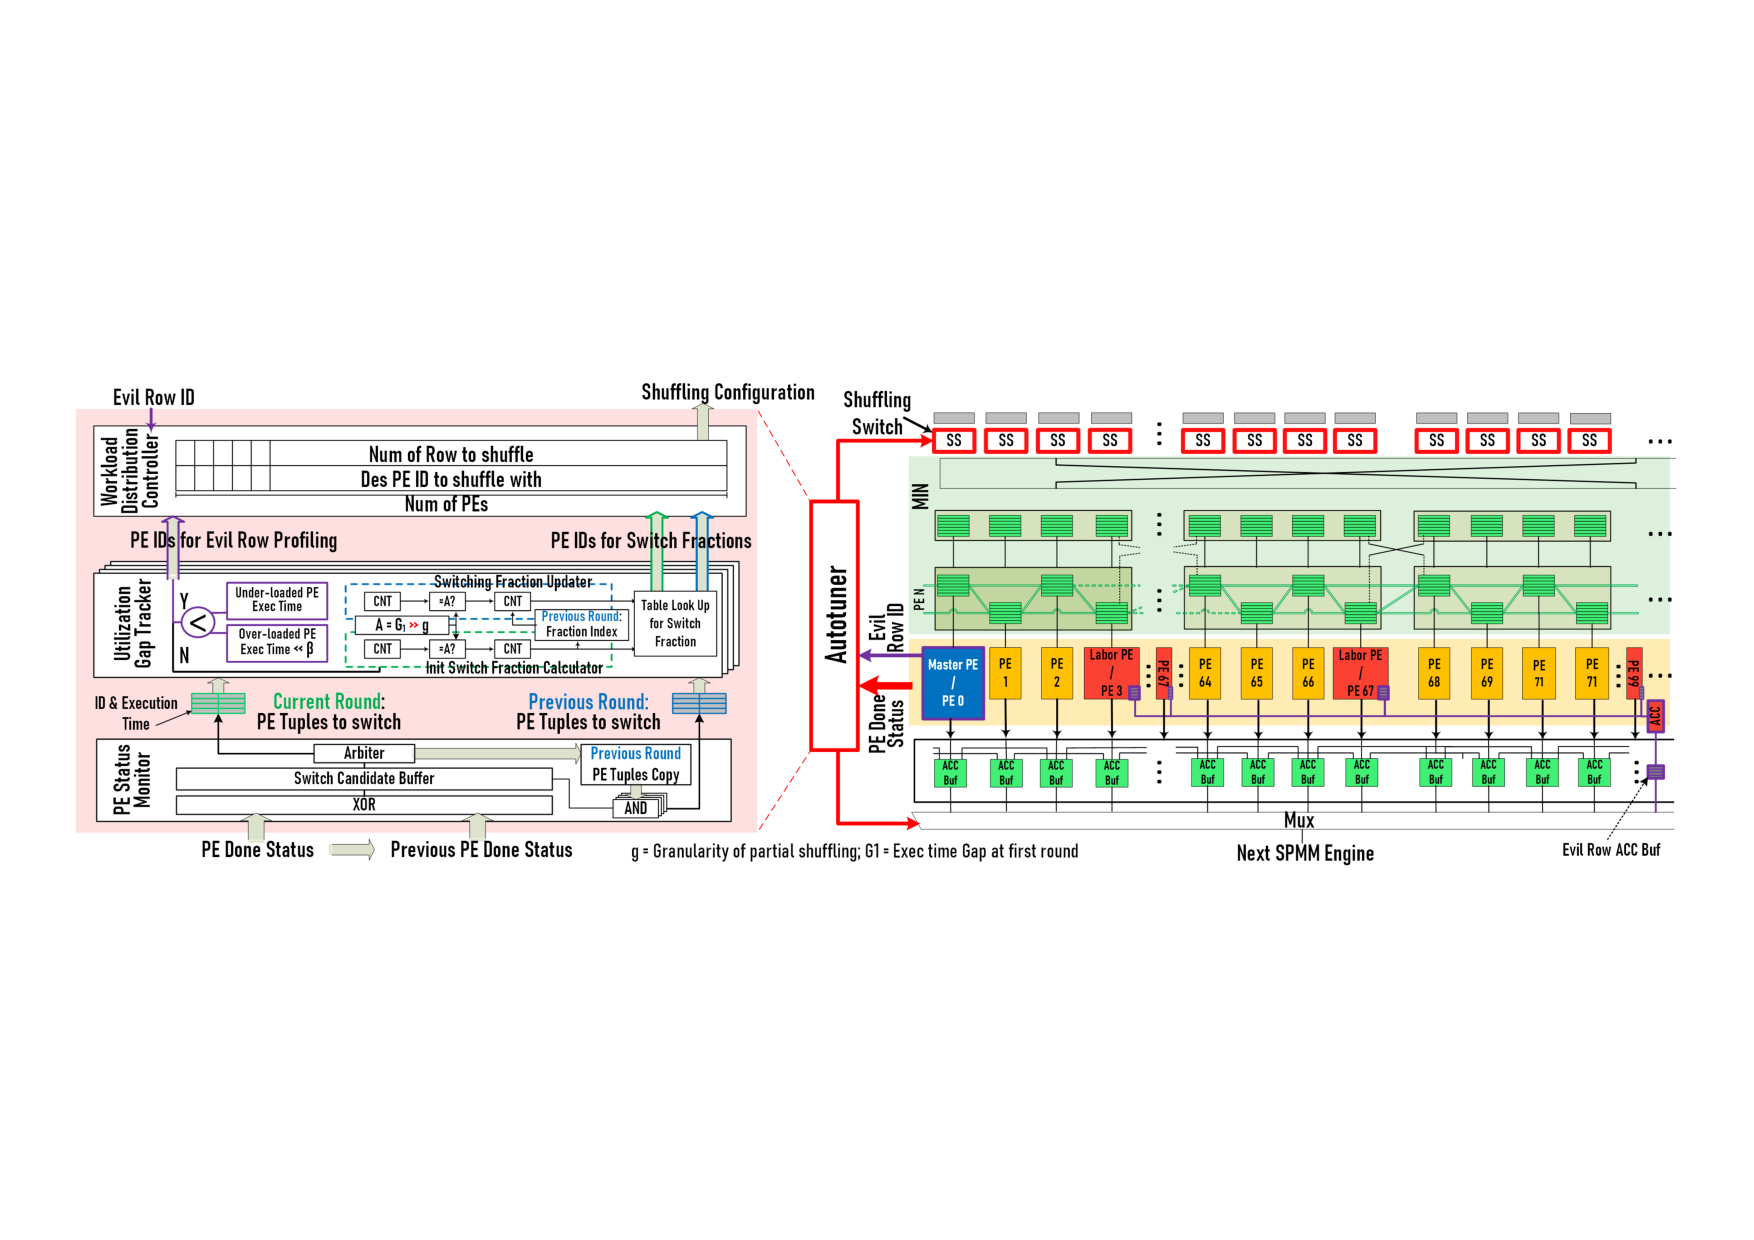
\includegraphics[height=0.28\textwidth]{Images/AWB_GCN_SpMM_architecture}
    \caption[Overall architecture of SpMM engine in AWB-GCN~\cite{DBLP:journals/corr/abs-1908-10834}]{Overall architecture of SpMM engine in AWB-GCN with three rebalancing techniques: distribution smoothing, remote switching (red bordered) and evil row remapping (purple bordered)~\cite{DBLP:journals/corr/abs-1908-10834}}
    \label{fig:awb_gcn_architecture}
\end{figure}

Specifically, AWB-GCN continuously monitors the sparse graph pattern, dynamically adjusts the workload distribution among many processing elements, and reuses the optimal configuration upon convergence.
Data from memory is directed through a task distributor and queue (TDQ) to a collection of processing elements (PEs) and accumulators.
The TDQ has two designs tailored for scenarios with moderate or high sparsity.
Given AWB-GCN's emphasis on GCNs featuring linear aggregation functions, the authors suggest prioritizing combination processing, as this typically reduces the number of features and subsequently minimizes the operations performed during aggregation.
Additionally, AWB-GCN incorporates a fine-grained pipelining mechanism to effectively overlap the execution of combination and aggregation, even within the same layer.

However, at the heart of the AWB-GCN architecture lies the management of load balancing at three levels of granularity: distribution smoothing to handle local utilization fluctuations among PEs, remote switching for minor crests, and row remapping for prominent crests.
At the beginning of the processing, rows are evenly distributed among processing elements.
Throughout each round of calculation, distribution smoothing equalizes the workloads among neighboring PEs.
The architecture of AWB-GCN effectively monitors the runtime PE utilization by tracking the number of pending tasks in task queues.
It continually offloads the work from more burdened PEs to their less occupied neighbors, up to 3-hop neighbors.

Remote switching is implemented to tackle regional clustering, wherein the process facilitates partial or complete workload exchanges between underutilized and overloaded PEs.
An auto-tuner dynamically determines the switch fraction at runtime, relying on the PE utilization observed in each round.
The accelerator retains the switch strategies employed in the current round and iteratively optimizes them based on utilization information gathered in the subsequent round.
As a result, after several rounds of auto-tuning, the switch strategy that best aligns with the sparse matrix structure is attained and is then utilized for the remaining rounds, leading to nearly perfect PE utilization.

Lastly, the evil-row remapping technique redistributes the evil row, i.e.\ a row of data that cannot be effectively smoothed or balanced through remote switching, to the most under-loaded PEs in troughs, allowing the neighboring PEs to assist.
Row remapping is initiated based on demand after each round.
The auto-tuner assesses the utilization gaps between the most overloaded and under-loaded PEs and decides if their gaps exceed remote switching capability.
If so, row remapping is executed as a solution.

AWB-GCN proves to be a fascinating accelerator, though its generalizability beyond Graph Convolutional Network remains uncertain.
On the other hand, EnGN~\cite{DBLP:journals/corr/abs-1909-00155} represents another accelerator featuring a unified architecture, with the primary goal of being adaptable for various Graph Neural Network models.

EnGN is a specialized accelerator architecture that prioritizes high-throughput and energy-efficient processing of large-scale GNNs in which the Graph Neural Network is treated as a concatenated matrix multiplication of feature vectors, adjacency matrices, and weights, all efficiently scheduled in a single data flow.
An array of clustered Processing Elements (PEs) is supplied with independent banks for features, edges, and weights, enabling computation of the combination function.
The hardware architecture of EnGN is shown in Figure~\ref{fig:engn_architecture}.

\begin{figure}[t]
    \centering
    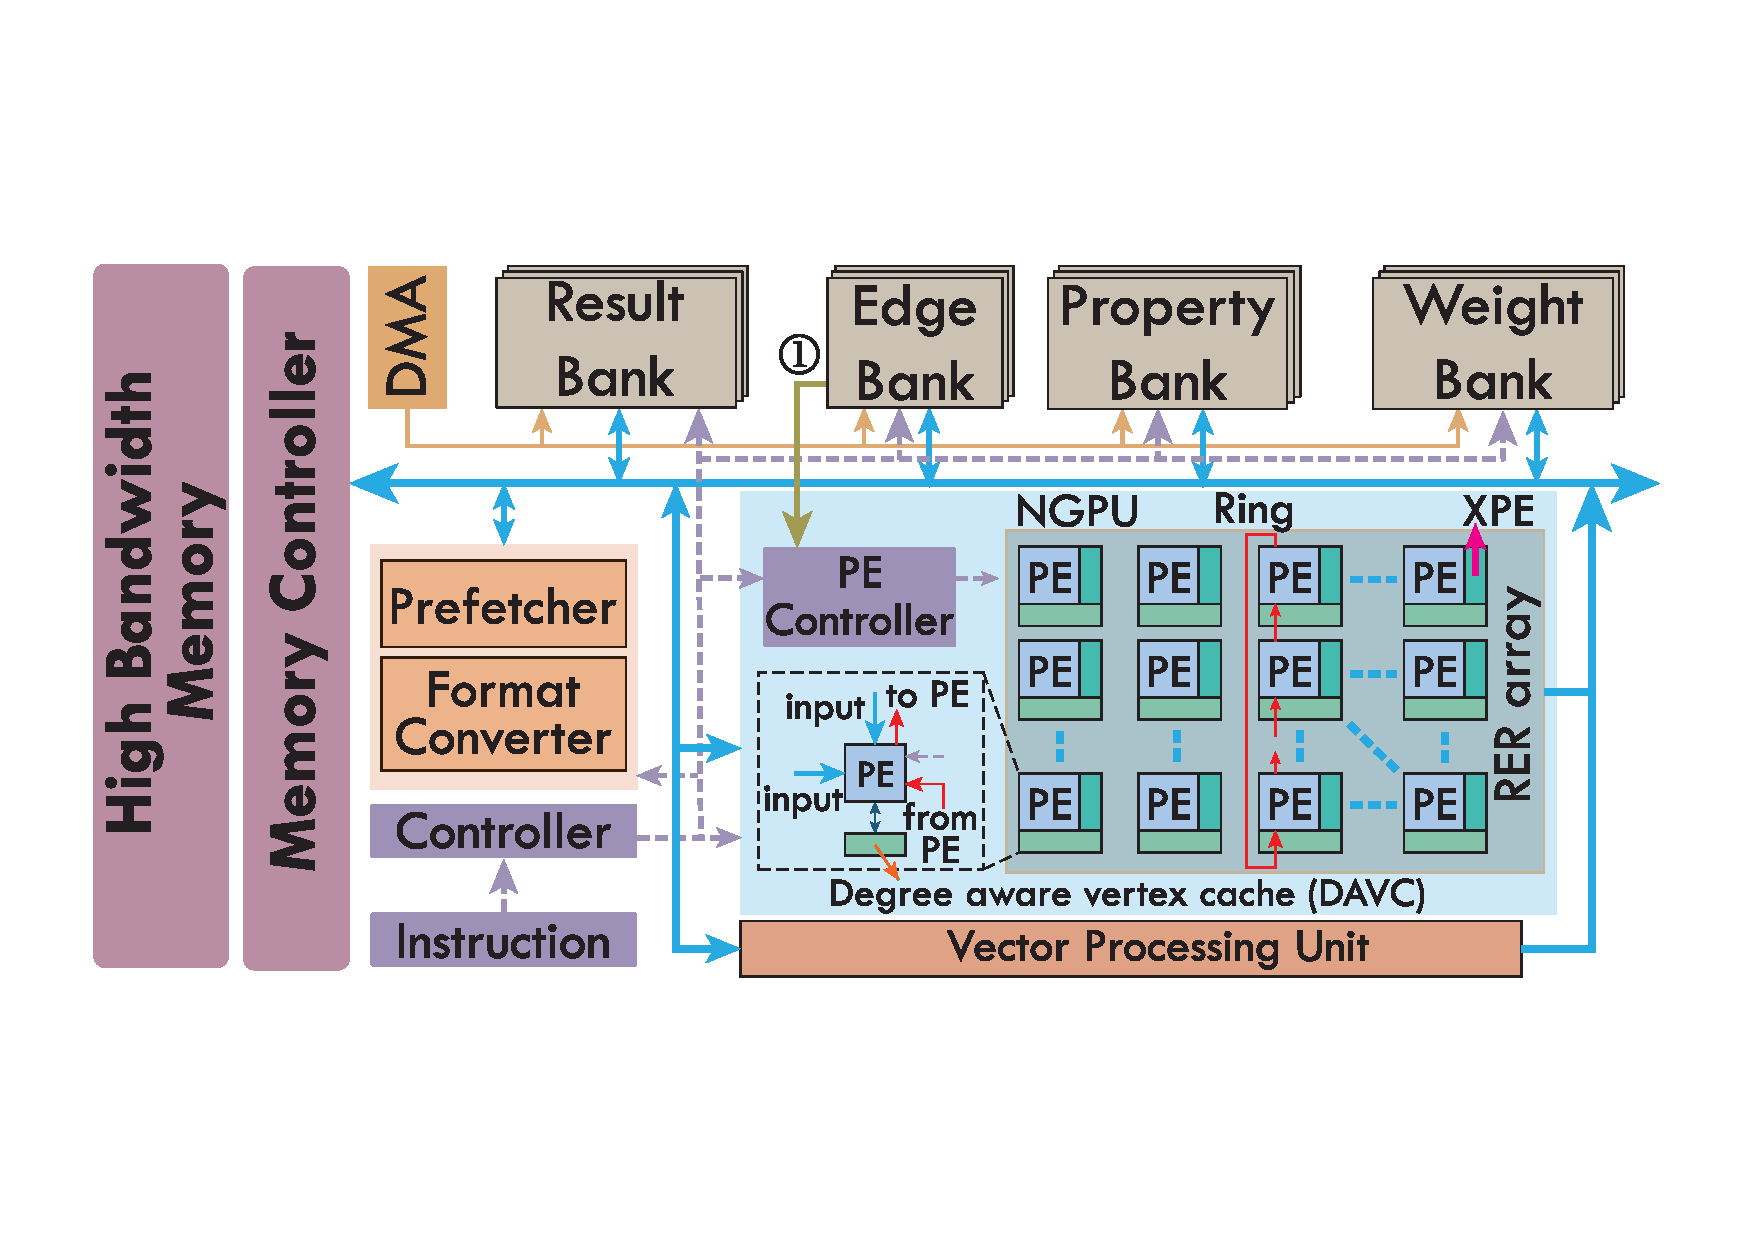
\includegraphics[height=0.3\textwidth]{Images/EnGN_architecture}
    \caption{EnGN hardware architecture~\cite{DBLP:journals/corr/abs-1909-00155}}
    \label{fig:engn_architecture}
\end{figure}

EnGN accelerates the three fundamental stages of GNN propagation to handle sparsity efficiently, i.e., feature extraction, aggregate, and update, which encapsulates common computing patterns shared by typical GNNs.
The authors introduce the ring-edge-reduce (RER) dataflow for the aggregation, in which each column of PEs is interconnected through a ring, and results are passed along and added based on the adjacency matrix.
This process effectively addresses the poor locality of sparsely and randomly connected vertices and efficiently supports critical stages.
EnGN dynamically reorders edges in each RER step to reduce redundant computations in sparsely connected nodes.

Since well-connected vertices frequently appear during computation, PE clusters have a degree-aware vertex cache that stores data for high-degree vertices.
Other optimized design decisions in EnGN involve the order of matrix multiplications when the aggregation function is a sum, impacting the total number of operations.

Moreover, EnGN employs a graph tiling strategy to accommodate large graphs, optimizing the utilization of hierarchical on-chip buffers through adaptive computation reordering and tile scheduling.
These optimizations collectively enhance the overall performance of EnGN for large-scale GNN processing tasks.

\subsection{GNN acceleration using Tiled architecture}
\label{subsec:tiled-architectures}%

A tiled architecture refers to a design approach where the FPGA fabric is organized into a regular grid-like pattern of configurable tiles.
Each tile typically consists of a set of logic cells, interconnect resources, and other functional units, and these tiles are repeated across the entire FPGA.

In contrast to most other accelerators, this work~\cite{9218751} presents a modular architecture for convolutional GNNs incorporating dedicated hardware units to efficiently handle the irregular data movement essential for graph computation in GNNs, while simultaneously delivering the high compute throughput required by GNN models.
The fundamental building block, as shown in the block diagram of Figure~\ref{fig:auten_tile_diagram} of the accelerator is a tile consisting of an aggregator module (AGG), a DNN accelerator module (DNA), a DNN queue (DNQ), and a graph PE (GPE), all interconnected via an on-chip router.

\begin{figure}[t]
    \centering
    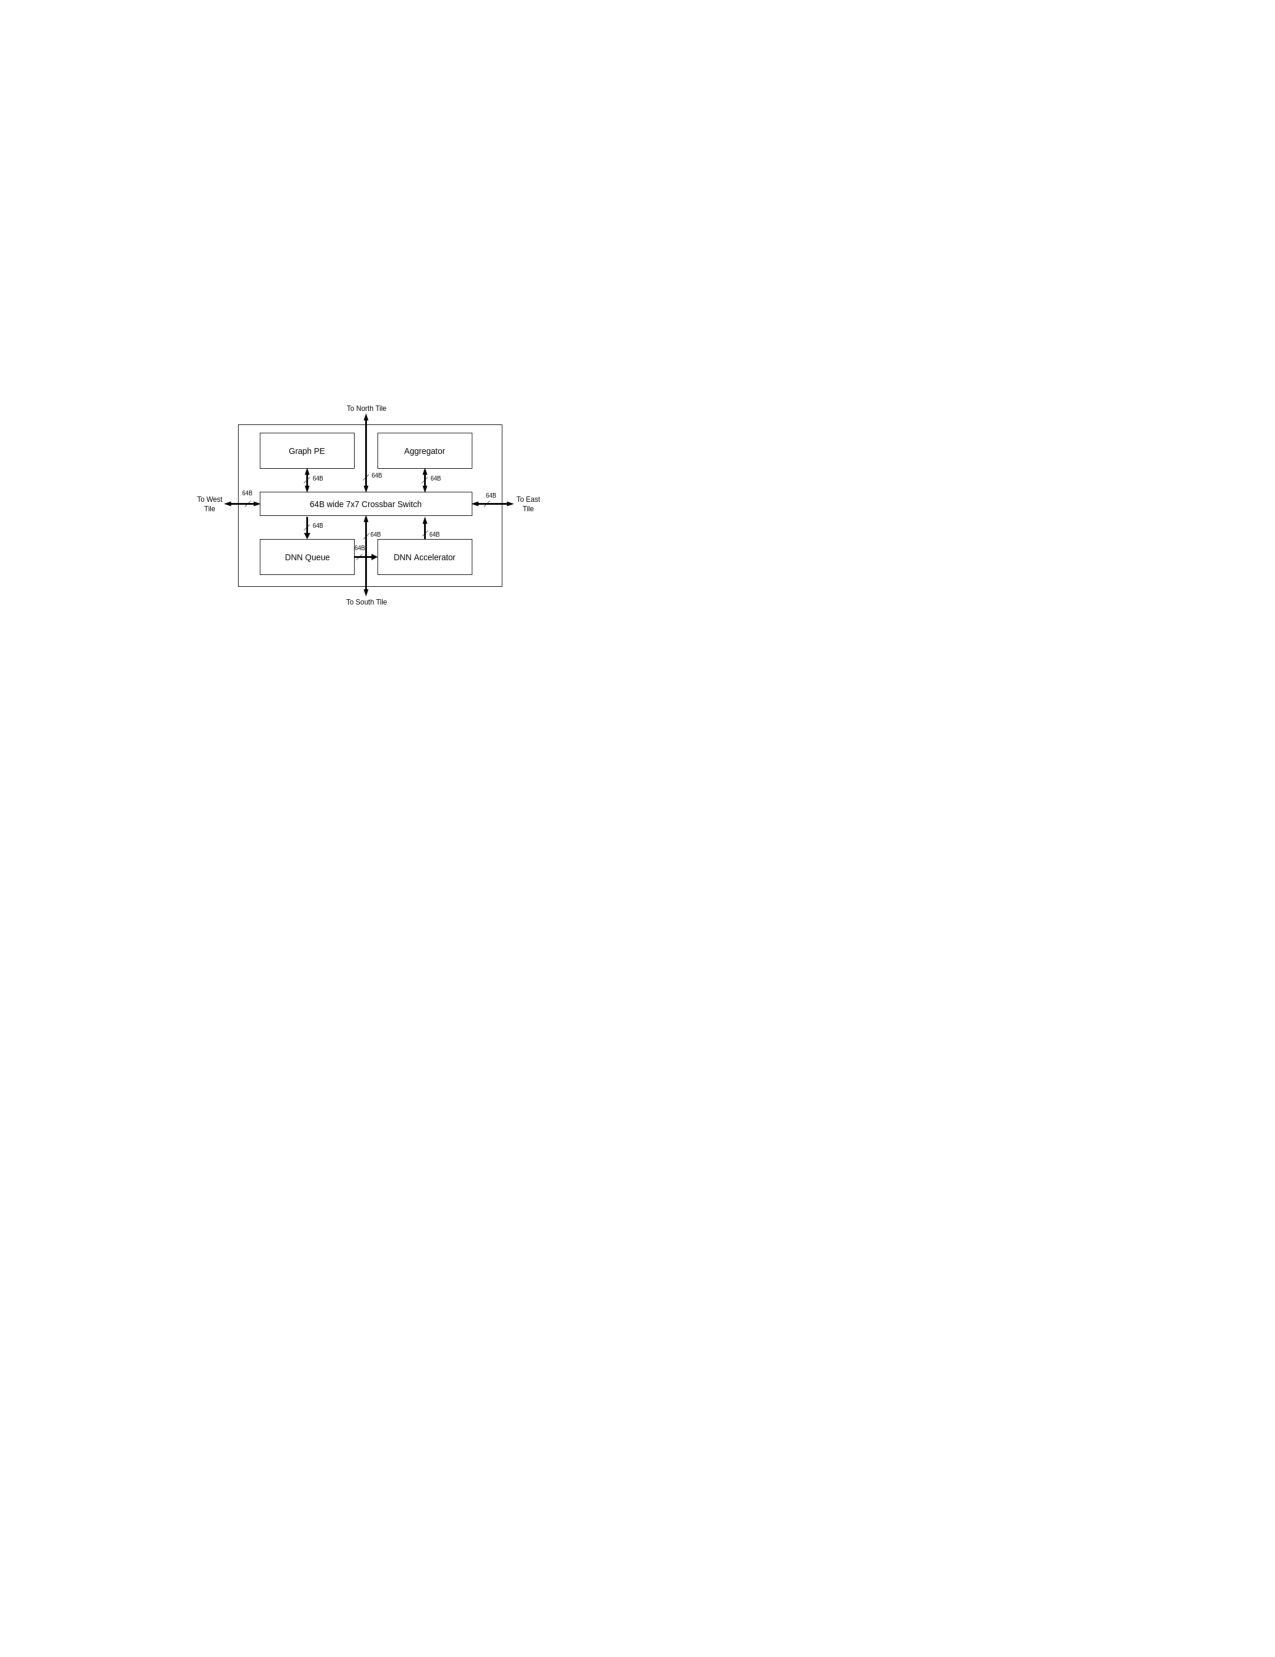
\includegraphics[height=0.3\textwidth]{Images/auten_tile_diagram}
    \caption{Block diagram of a tile in the GNN accelerator proposed by Auten \textit{et al.}~\cite{9218751}}
    \label{fig:auten_tile_diagram}
\end{figure}

The Graph Processing Element (GPE) handles graph traversal and sequencing computation steps dependent on the underlying graph structure.
The DNA executes the DNN computation within the GNN model.
The AGG performs feature aggregation coordinated by the GPE based on graph traversal.
The DNQ buffers memory requests and intermediate results as they are passed to the DNA.
This design allows for easy scalability by interconnecting multiple tiles with memory.

The GNN accelerator program proposed by Auten \textit{et al.}~\cite{9218751} represents a GNN model as a sequential set of layers.
Each layer operates on a graph, applying a vertex program to generate an output graph.
These layers are connected in sequence to form a complete GNN model.
The initial layer takes the model input as its input graph, and subsequent layers utilize the output of the preceding layer.
The last layer produces the final output graph.

\subsection{Hybrid architectures for GNN acceleration}
\label{subsec:hybrid-architectures}%

HyGCN~\cite{DBLP:journals/corr/abs-2001-02514} is a unique GCN accelerator due to its innovative hybrid architecture.
This approach was inspired by the observation that GNNs exhibit two distinct execution patterns with contrasting requirements: the aggregation phase involves graph processing, displaying a dynamic and irregular execution pattern.
On the other hand, the combination phase behaves more like conventional neural networks, exhibiting a static and regular execution pattern.
As a result of this observation, HyGCN consists of dedicated engines for the aggregation and combination stages and a coordinating mechanism for pipelined execution of both functions.

The Combination operation at each vertex works like a neural network with a regular yet compute-intensive execution.
HyGCN's architecture is based on the popular systolic array, but it incorporates multiple arrays instead of a single one to adapt to the two processing modes of the Aggregation Engine.
In the combination engine, a set of systolic arrays is combined to form a systolic module, and these modules can be flexibly utilized in various ways, including independent and cooperative working modes.

In the independent working mode, the systolic modules operate autonomously, each handling the matrix-vector multiplication (MVM) operations of a small group of vertices.
This mode offers the benefit of reduced vertex latency since the Combination operations for this smaller group of vertices can be processed immediately once their aggregated features are ready without waiting for additional vertices.
In the cooperative working mode, a large group of vertices' aggregated features are gathered and combined.
The advantage of this mode is that weight parameters can be efficiently reused by all systolic arrays, reducing energy consumption.

The aggregation engine, represented in Figure~\ref{fig:hygcn_architecture}, comprises a sampler, edge scheduler, and sparsity eliminator feeding a set of SIMD (single instruction multiple data) cores.
There are two processing modes for SIMD cores to handle edges in parallel.

\begin{figure}[t]
    \centering
    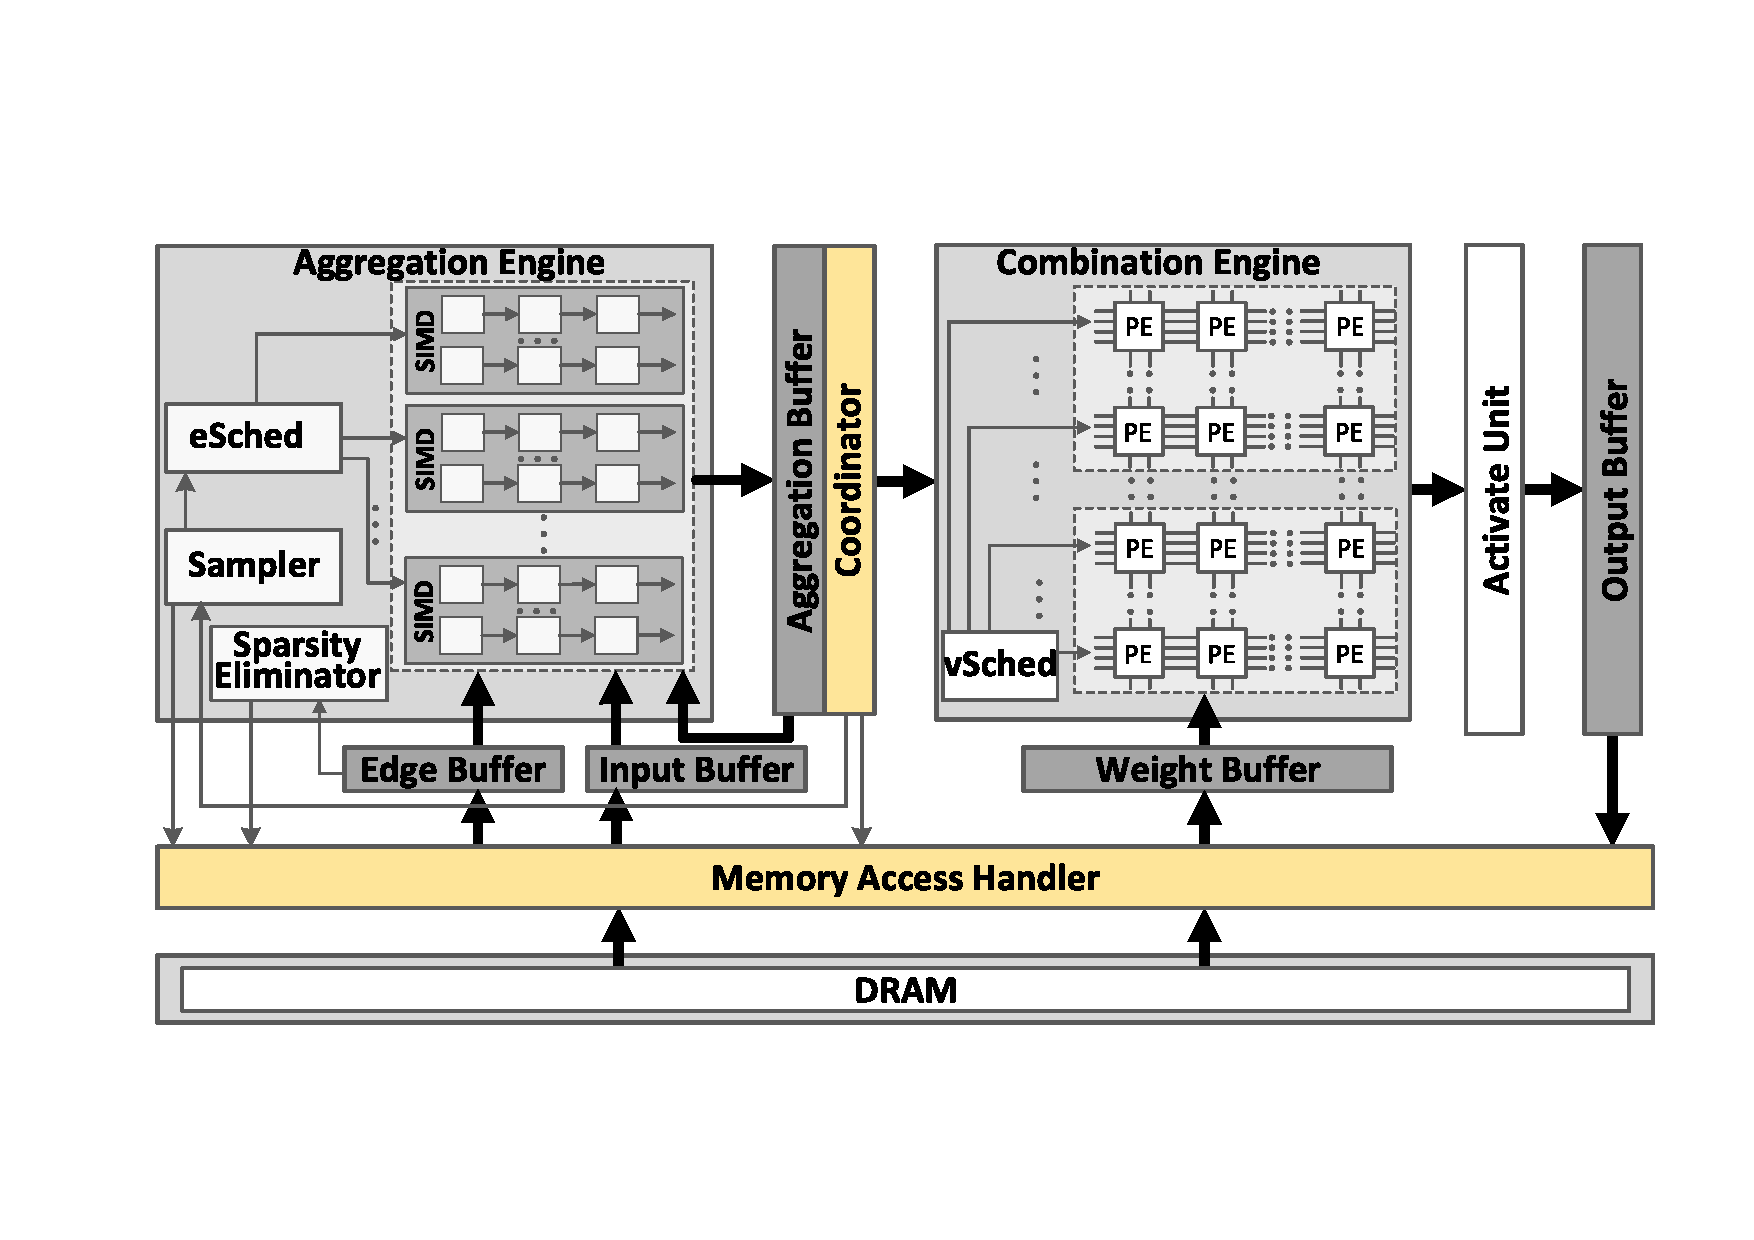
\includegraphics[height=0.3\textwidth]{Images/HyGCN_architecture}
    \caption{Architecture overview of HyGCN~\cite{DBLP:journals/corr/abs-2001-02514}}
    \label{fig:hygcn_architecture}
\end{figure}

The first mode is vertex-concentrated, where each SIMD core is assigned the workload of a single vertex.
While this mode can produce aggregated features in a burst mode, the processing latency for a single vertex is prolonged, leading to workload imbalance and loss of parallelism.
On the other hand, the vertex-disperse processing mode assigns the aggregation of elements in the vertex feature vector to all cores.
This mode ensures that all cores are constantly busy without workload imbalance.
Additionally, it enables immediate processing of each vertex in the subsequent Combination Engine while reducing the latency for a single vertex compared to processing multiple vertices together.
To enhance the computation of aggregation, HyGCN uses the vertex-disperse processing mode.

HyGCN utilizes a static graph partition method to optimize memory access to improve data reuse.
The authors identified that the feature vectors of each vertex are typically large, making the exploitation of feature locality crucial.
To address this, they grouped vertices in disjoint sets and processed the aggregation of their source neighbors group by the group.
By following this approach, the feature accesses of all vertices in an interval were merged.
This grouping allowed for overlapping neighbors within the considered interval, enabling the reuse of loaded feature data during feature aggregation.
Moreover, when traversing all the neighbors of the interval, the intermediate aggregated results of the grouped vertices were stored in a buffer and could be reused during feature updates.

Sparsity is efficiently handled at the aggregation engine through effective scheduling and the sparsity eliminator, which adapts dynamically to varying degrees of sparse multiplications using a window-based sliding and shrinking approach.
In particular, the authors implemented this approach to enhance data reuse and minimize redundant accesses caused by sparse graph connections.
The central idea was to slide the window downward until an edge appeared in the top row and then shrink its size by moving the bottom row upward until an edge was encountered.
This method effectively eliminated sparsity and improved data access efficiency.

To further optimize for varying workloads, HyGCN allows flexible grouping of SIMD cores in aggregation and PEs in combination based on the size of feature vectors.
Additionally, careful attention is given to the design of the inter-engine coordinator to optimize memory accesses and enable fine-grained pipelining of execution, maximizing parallelism dynamically.

The internal structure of each tile in the accelerator proposed in~\cite{9218751} resembles HyGCN's, with the DNA functioning as an array for dense multiplication, the AGG as an edge-controlled adder, the DNQ as an inter-engine buffer, and the GPE overseeing execution.
Unlike HyGCN, the accelerator introduced in~\cite{9218751} is less specialized and has a better potential for generalization to various Graph Neural Network models~\cite{DBLP:journals/corr/abs-2010-00130}.

While not an authentic hybrid architecture, GRIP~\cite{DBLP:journals/corr/abs-2007-13828} is an accelerator that shares similar techniques with HyGCN's implementation approach.
It leverages GReTA~\cite{greta-recoml20} (Gather, Reduce, Transform, Activate), a graph processing abstraction specifically crafted for efficient execution on accelerators.
It also offers the flexibility required to implement GNN inference and holds the potential to be adaptable to various types of Graph Neural Networks.

GRIP is an accelerator designed to achieve low-latency inference.
It addresses the challenges of accelerating GNNs, combining two distinct computation types: arithmetic-intensive vertex-centric operations and memory-intensive edge-centric operations.
To tackle this, the accelerator divides GNN inference into fixed sets of edge- and vertex-centric execution phases, making them suitable for hardware implementation.
Each unit is then specialized to handle the unique computational structure of each phase efficiently.

GRIP utilizes a high-performance matrix multiply engine and a dedicated memory subsystem for vertex-centric phases for weights to enhance data reuse.
In contrast, it employs multiple parallel prefetches and reduction engines for edge-centric phases to mitigate the irregularity in memory accesses.
Additionally, GRIP supports several GNN optimizations, including a novel technique called vertex-tiling, which enhances the reuse of weight data.

GRIP provides a customizable architecture, shown in Figure~\ref{fig:grip_architecture}, with separated and custom units and accumulators for both edges (gather, reduce) and vertices (transform, activate) that allows for performing edge and node updates using user-defined functions.
The control of GRIP is managed by a host system that issues commands for different operations and data transfers.
The control unit dequeues these commands in order and asynchronously issues them to individual execution units or the memory controller.

\begin{figure}[t]
    \centering
    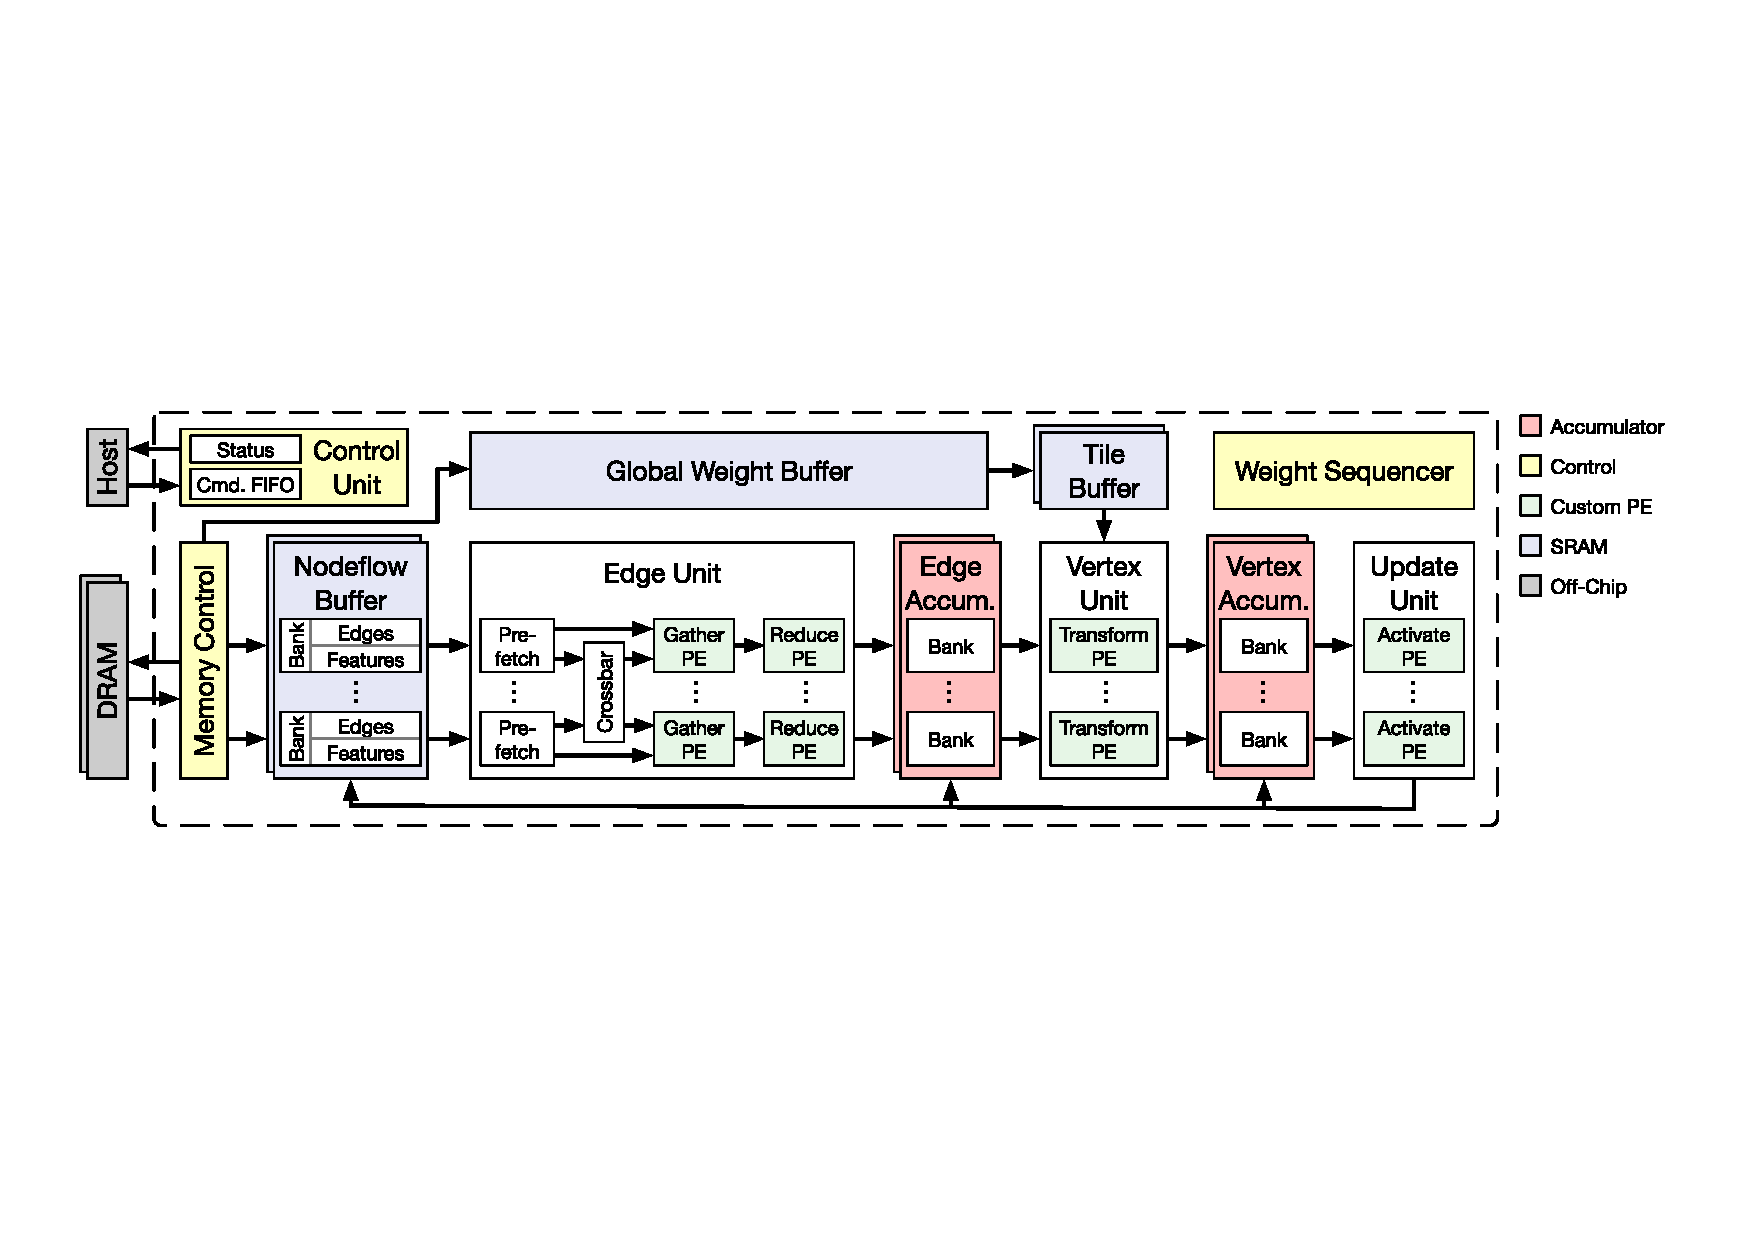
\includegraphics[height=0.26\textwidth]{Images/GRIP_architecture}
    \caption{High-level overview of GRIP~\cite{DBLP:journals/corr/abs-2007-13828}}
    \label{fig:grip_architecture}
\end{figure}

GRIP comprises three core execution units: the edge unit, the vertex unit, and the update unit.
The edge unit performs the edge-accumulate phase, iterating over the edges of the nodeflow, executing gather, and accumulating the result into the edge accumulator using reduce.
The vertex unit performs the vertex-accumulate phase, iterating over the output vertices corresponding to the accumulated edge values, executing the transform, and accumulating the result into the vertex accumulator.
The update unit performs the vertex-update phase, reading the accumulated values for each vertex and passing them to the activated PE.
The result is then written to the nodeflow buffer as an updated feature or to the edge or vertex accumulator, enabling efficient data flow between different GRIP programs when executed in sequence.

As already said, GRIP allows users to customize the four PEs, which can be implemented in multiple ways based on their specific requirements.
In the authors' implementation, a programmable ALU-based approach is used, splitting the edge update unit into lanes to execute vertices simultaneously.
It adopts an input-stationary dataflow for the vertex update unit.
The accelerator employs various optimizations, including pipelining and tiling adapted to the specific dataflows implemented, similar to other accelerators.

\subsection{Challenges}
\label{subsec:hw-accelerators-discussion}%

This section presented a variety of GNN hardware accelerators, but despite many alternatives, there is still the need to face some open challenges.
In particular, most of the presented solutions target only specific models of GNNs, and it is unclear how to generalize them.

Hardware accelerators face the challenge of striking the appropriate balance between performance and generalization, considering the multitude of graph types and GNN variants.
Moreover, the wide variety of problems, each with varying graph and feature vector sizes, increases the complexity of the acceleration task.

Given that the field of GNN accelerators is constantly evolving, researchers are actively investigating innovative architectural and algorithmic solutions.
This thesis aims to introduce a novel GNN accelerators design technique that can be tailored to specific requirements, offering an alternative to existing solutions with the advantage of a faster and automated design.

\section{High-Level Synthesis based accelerators}
\label{sec:hls-accelerators}%

As previously highlighted, one of the main challenges of GNN hardware acceleration lies in simultaneously meeting the demand for supporting novel GNN models and fast inference, as there exists a gap between the development time of efficient FPGA accelerators and the rapid evolution of new GNN models.

Unlike the designs presented in the previous section, typically designed using low-level hardware description languages by explicitly specifying the hardware components and their interconnections, this section discusses methods to generate accelerators using HLS, which automatically synthesizes high-level code into hardware, abstracting away low-level hardware details.

GenGNN~\cite{DBLP:journals/corr/abs-2201-08475} is a GNN acceleration framework utilizing High-Level Synthesis, with two primary objectives.
Firstly, to achieve ultra-fast GNN inference without needing graph pre-processing to meet real-time demands.
Secondly, to support a wide range of GNN models with the flexibility to accommodate new models.
The framework incorporates an optimized message-passing structure that applies to all models and is complemented by a diverse library of model-specific components.

This framework capitalizes on the observation that each node in a GNN layer undergoes two key steps: message passing (MP) and node embedding (NE). The message passing step is further divided into gather and scatter phases, where gather involves feature aggregation, and scatter entails message transformation and forwarding.
On the other hand, node embedding encompasses node transformation and update.

To accelerate MP and NE steps, GenGNN was designed using a message-passing style featuring two main processing elements (PEs): node embedding and message passing.
As shown in Figure~\ref{fig:gengnn_architecture}, the architecture includes three data storage buffers: one node embedding buffer and two message buffers, all of which have a $O(N)$ size, where $N$ represents the number of nodes allowed on-chip.
The two message buffers are used alternately across layers, allowing for the reuse of resources and dataflow in multiple layers.
The node embedding PE handles node transformation and update within a single layer, while the message passing PE performs the subsequent scatter operation.
The advantage of this approach is that the receivers of the messages can instantly update their partially aggregated message in the message buffer, enabling the merging of scatter and gather phases.
Since the aggregation function is permutation invariant and the aggregation order does not matter, such a merged fashion reduces the overall process latency and minimizes memory cost.

\begin{figure}[t]
    \centering
    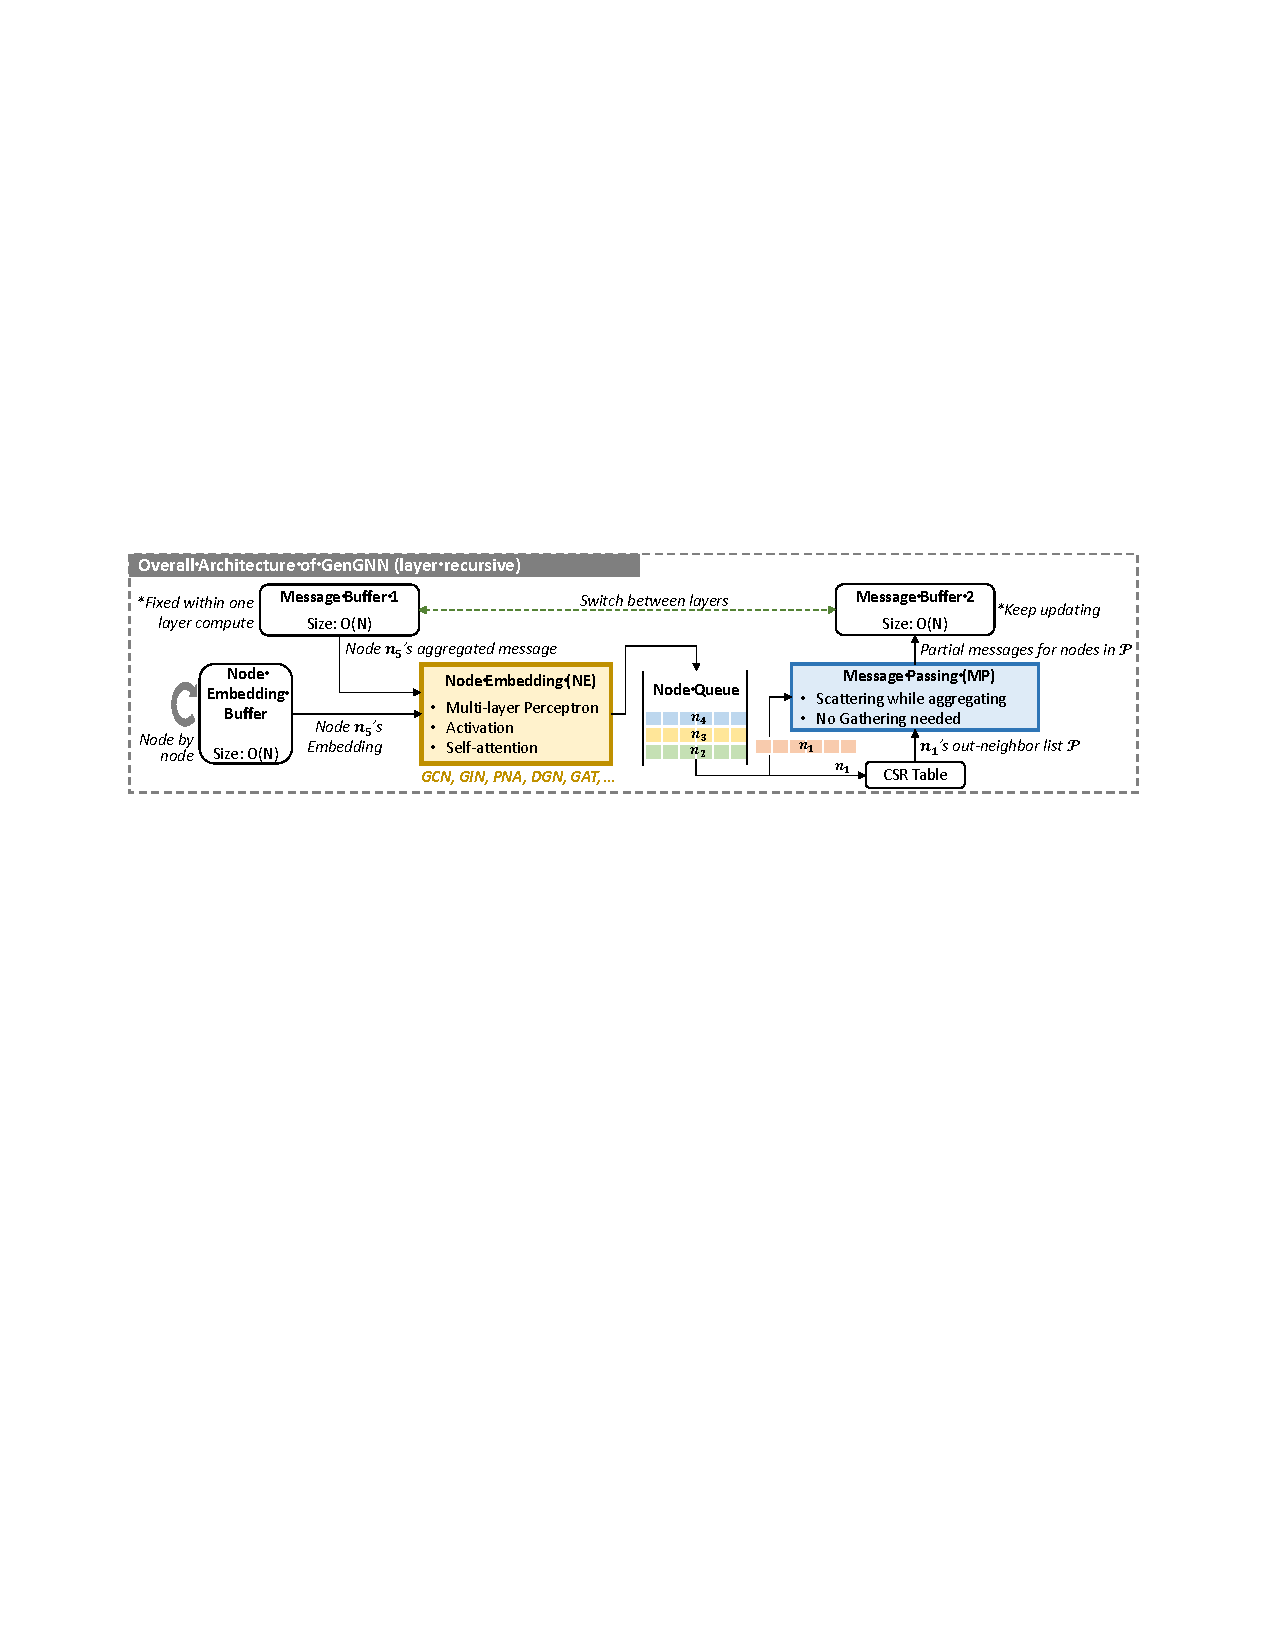
\includegraphics[height=0.22\textwidth]{Images/GenGNN_architecture}
    \caption{GenGNN overall architecture~\cite{DBLP:journals/corr/abs-2201-08475}}
    \label{fig:gengnn_architecture}
\end{figure}

The independence of node embedding (NE) and message passing (MP) steps across nodes and edges allows for significantly reduced processing latency by effectively pipelining these two steps.
The authors referred to the most suitable approach for this task as streaming-based pipelining, which can be achieved using a streaming-based FIFO (first-in-first-out) memory queue.
In this implementation that significantly reduces idle cycles and minimizes resource usage, NE and MP are pipelined flexibly using a node queue.
Once a node completes its NE and is prepared for message passing, its embeddings are pushed into the queue.
At the same time, the MP engine reads from the queue, fetching the node embeddings for message passing.

GenGNN enhances its architecture's adaptability to different graph neural network models by offering various model-specific components.
One particularly advantageous feature of GenGNN's streaming-based pipelining for node/edge processing is its suitability for models with virtual nodes.
As defined by~\cite{DBLP:journals/corr/GilmerSRVD17}, a virtual node acts as an artificial node connected to all other nodes in the graph, creating a shortcut for message passing between node pairs.
The authors stated that processing the virtual node can be entirely overlapped with the node embedding computation for other nodes, ensuring zero waste as long as it is handled early enough in the processing pipeline.

Finally, another feature provided by GenGNN is the large graph extension.
The authors implemented a prefetcher to accommodate large graphs that cannot be stored on-chip.
This prefetcher retrieves consecutive nodes' degrees from DRAM and stores them in an on-chip FIFO buffer.
As the message passing PE requires, it loads each subsequent node's degree, prompting the prefetcher to refill the buffer.
This clever mechanism effectively conceals the latency associated with fetching from the off-chip degree table, ensuring that the message passing PE behaves similarly to handling small graphs.
Moreover, the authors adopted packed data transfer by typecasting off-chip array pointers into the desired size pointer types, facilitating the transfer of more significant bits between DRAM and the system with every clock cycle.

Another notable framework in this section is DGNN-Booster~\cite{chen2023dgnnbooster}, an innovative Field-Programmable Gate Array accelerator framework designed for real-time inference of Dynamic Graph Neural Networks (DGNNs) using High-Level Synthesis.
Unlike the other accelerators mentioned and outside the scope of this research, DGNN-Booster focuses on DGNNs, which are Graph Neural Networks tailored for dynamic graph structures and features.
However, it is worth mentioning that DGNN-Booster implements GNNs using a message-passing mechanism based on GenGNN at a lower level of parallelism.

\section{Software-Hardware co-design accelerators}
\label{sec:software-hardware-accelerators}%

Software-hardware co-design is an integrated approach which involves designing both software and hardware components collaboratively to enhance system performance and efficiency.
Unlike traditional design methods where software and hardware are developed independently and later integrated, co-design seeks to unify these two elements from the beginning of the design process.
This design strategy evaluates which tasks are suitable for offloading to software and which should remain in hardware, considering the associated overheads.

The work conducted by Zhang \textit{et al.}~\cite{9153263} introduces a combined software and hardware approach for accelerating Graph Convolutional Networks.
Their study was initiated with the recognition that hardware acceleration of Graph Convolutional Network inference poses challenges stemming from the vast size of the input graph,
the heterogeneous workload of GCN inference involving sparse and dense matrix operations, and the irregular information propagation along the edges during computation

The primary objective of this accelerator is to accelerate GCN models, with a particular focus on the critical computational kernels: feature aggregation $AX$ and feature transformation $XW$.
In these kernels, $A$ represents the adjacency matrix, $X$ denotes the feature matrix, and $W$ represents the weight matrix.

The proposed algorithm-architecture co-optimization for accelerating large-scale Graph Convolutional Network inference on FPGA involves several key steps.
First, the authors implemented a data partitioning scheme for GCN inference to accommodate real-world datasets with huge dimensions for $A$ and $X$.
This approach ensures that both the adjacency matrix and the feature matrix can fit on-chip while mapping the computational kernels onto the FPGA\@.

Then, the graph undergoes a two-phase preprocessing algorithm involving sparsification and node reordering. 
The sparsification phase eliminates edge connections of high-degree nodes by merging familiar neighbors to reduce the memory accesses that a graph with more edges can require during the aggregation stage.
The node reordering phase effectively groups adjacent nodes to enhance on-chip data reuse.

\begin{figure}[t]
    \centering
    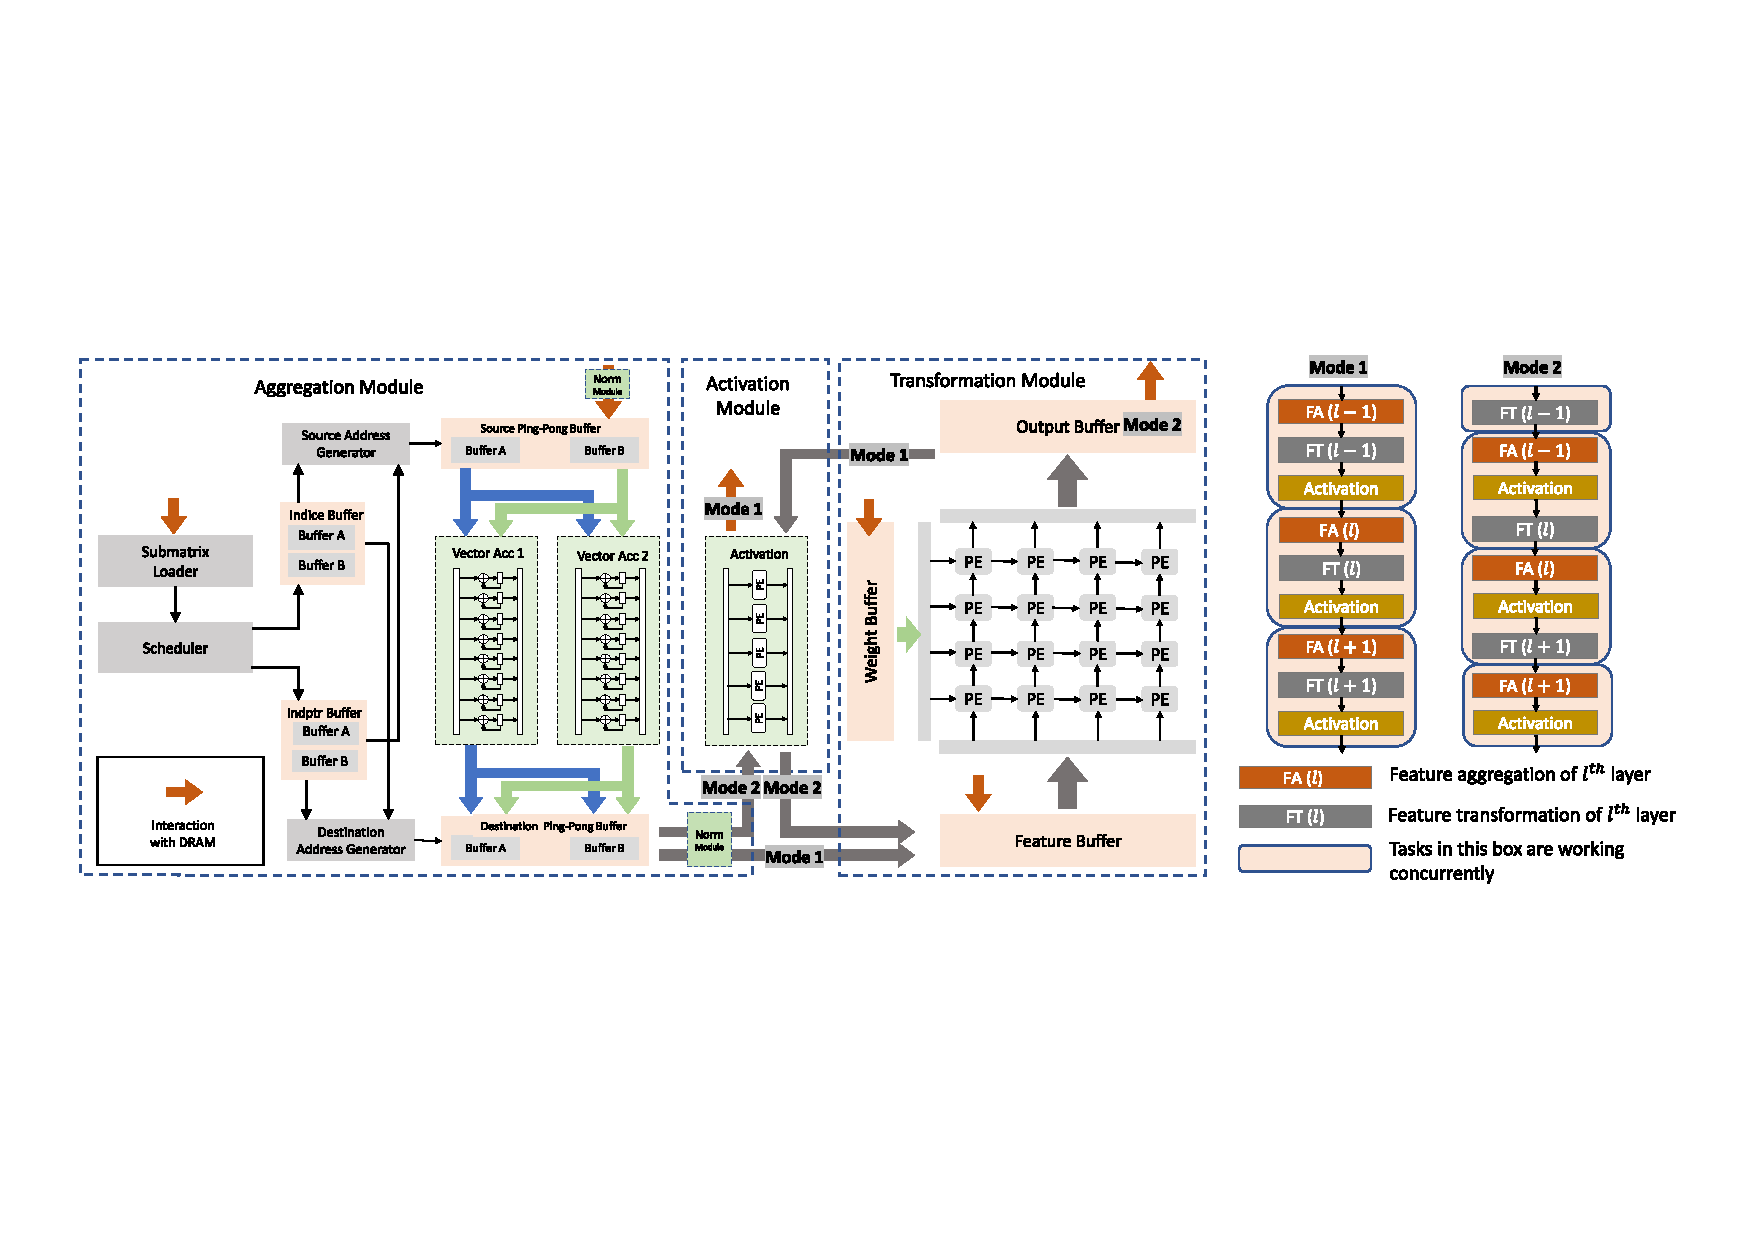
\includegraphics[height=0.26\textwidth]{Images/zhang_architecture}
    \caption{Hardware architecture with two execution modes proposed by Zhang \textit{et al.}~\cite{9153263}}
    \label{fig:zhang_architecture}
\end{figure}

The pre-processed graph is then fed into a hardware accelerator implemented in an FPGA that efficiently pipelines GCN's two major computational kernels: aggregation and transformation.
As outlined in~\cite{DBLP:journals/corr/abs-2010-00130}, the design, shown in Figure~\ref{fig:zhang_architecture}, distinguishes itself from other approaches in several ways.
The aggregator module adopts a double-buffering technique to hide addition latency and leverages node- and feature-level parallelism.
Moreover, the accelerator supports two modes of operation depending on the order of matrix multiplications, leading to different pipelining strategies.
In order to accommodate these modes, the modules are interconnected from the aggregate module to the combination modules and vice versa.

GenGNN's NE/MP pipeline, introduced in Section~\ref{sec:hls-accelerators}, shares a similar concept with the task scheduling approach of BoostGCN~\cite{9444065}.
BoostGCN presents a framework, shown in Figure~\ref{fig:boost-gcn-framework}, using an algorithm-architecture co-optimization scheme tailored to enhance GCN inference on FPGA.
The authors introduced a groundbreaking hardware-aware Partition-Centric Feature Aggregation (PCFA) scheme that capitalizes on 3-D partitioning alongside the vertex-centric computing paradigm.
This innovation significantly boosts on-chip data reuse while minimizing the overall data communication volume with external memory.

Furthermore, they devised a novel hardware architecture that enables seamless pipelined execution of the computation phases of inference: feature aggregation and feature update.
They developed a low-overhead task scheduling strategy to tackle any potential pipeline stalls arising from these phases.

The authors delivered a comprehensive GCN acceleration framework on FPGA, complete with meticulously optimized RTL (Register-Transfer Level) templates.
This framework can generate hardware designs based on personalized configurations and is adaptable to diverse GCN models.
BoostGCN's overall system architecture comprises external memory and FPGA components.
Feature Aggregation Modules (FAMs) handle feature aggregation on the FPGA board, while Feature Update Modules (FUMs) manage feature updates.
Intermediate results generated by FAMs are cached in the Internal Buffer, and the Memory Controller manages data transmissions between external memory and hardware modules.

The authors propose a specific approach to optimize task scheduling and minimize pipeline stalls for FUM and FAM. This involves arranging intervals based on their vertex degrees and prioritizing intervals with more minor vertex degrees for execution first.
Furthermore, they allocate a buffer in external memory to store aggregated feature vectors produced by FAMs in case FUM is not yet prepared to consume new aggregated feature vectors.
Subsequently, FUM can retrieve the aggregated feature vectors from external memory when ready.

As indicated in~\cite{DBLP:journals/corr/abs-2201-08475}, while the scheduling approaches of GenGNN and BoostGCN share some similarities, there are notable differences.
Firstly, BoostGCN relies on sorting vertices by degrees on the CPU to establish an execution order, whereas GenGNN processes the nodes on-the-fly in FPGA in an adaptive manner.
Secondly, BoostGCN employs a buffer in external memory, while GenGNN utilizes an on-chip FIFO to queue the nodes ready for message passing.

\begin{figure}[t]
    \centering
    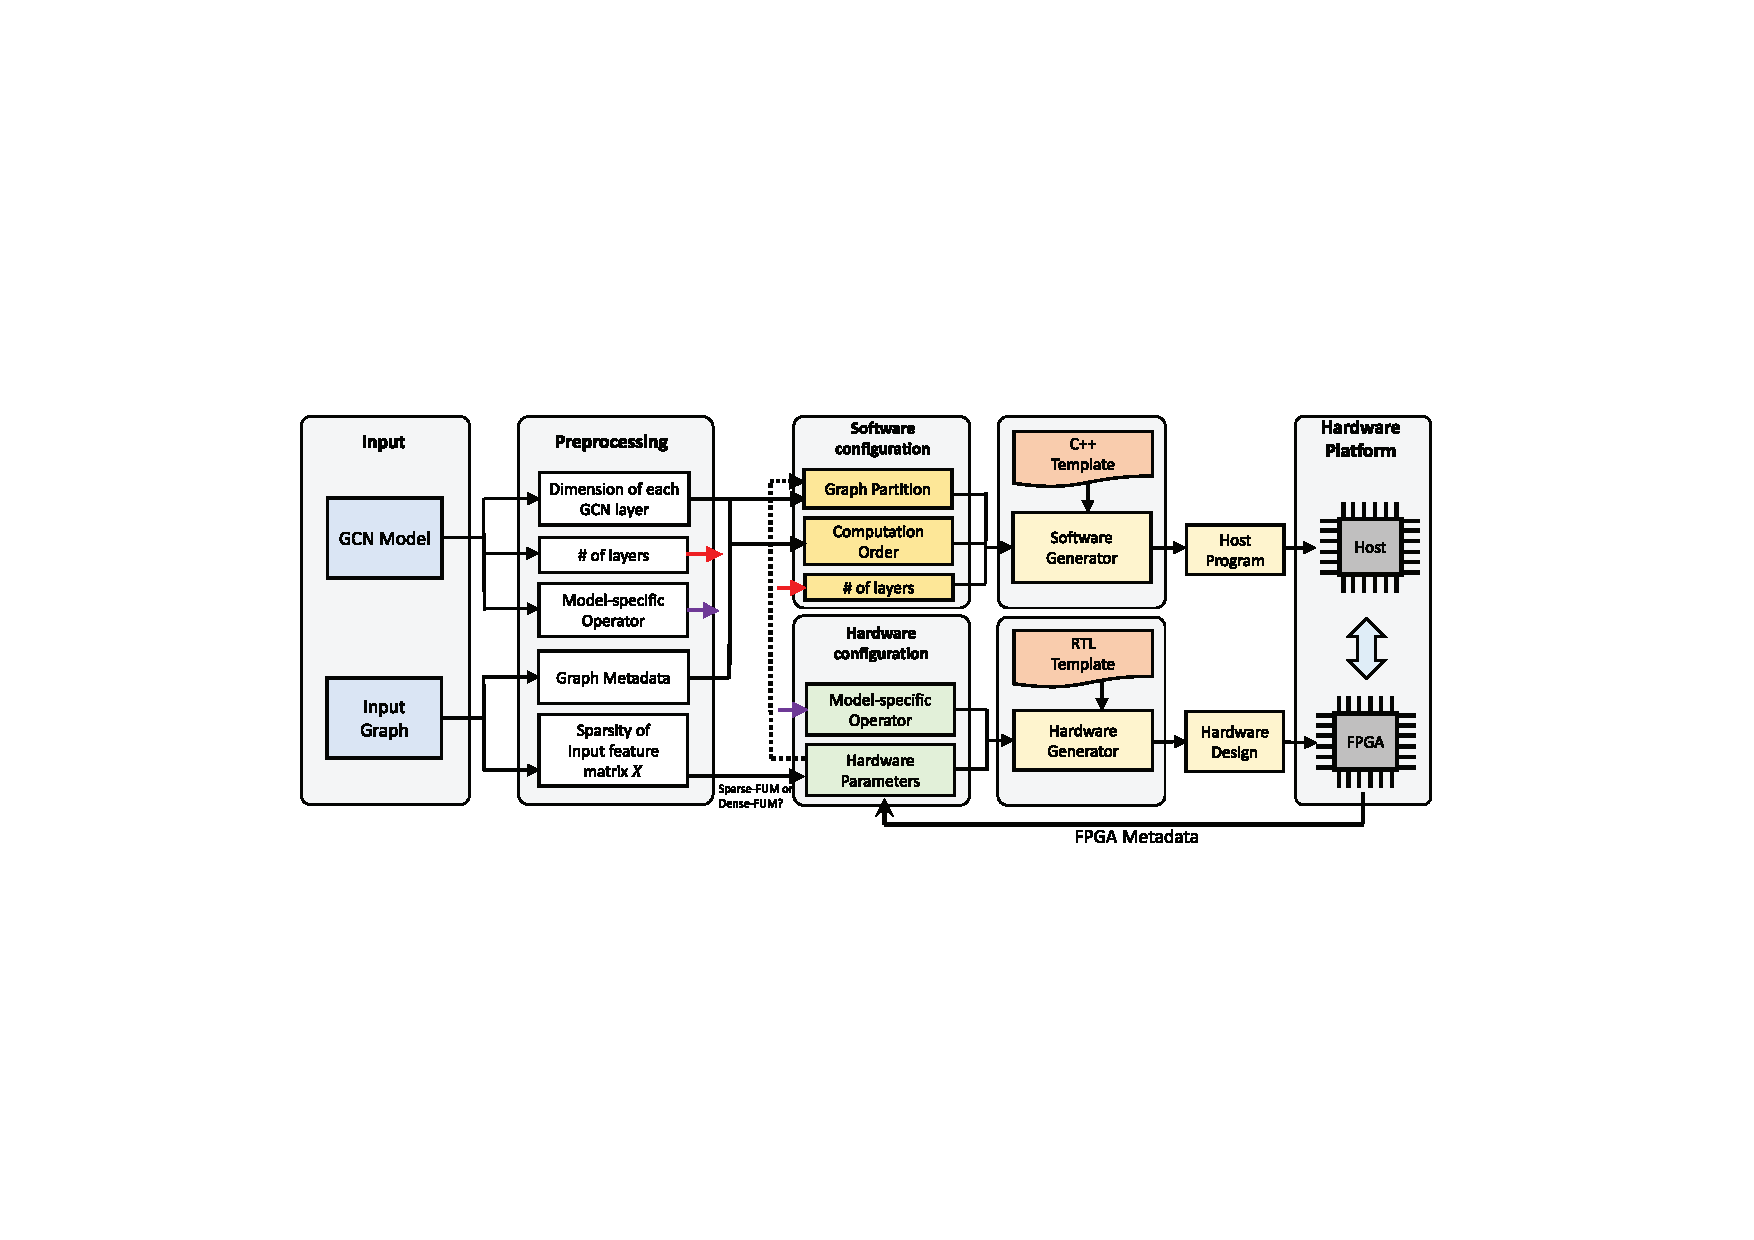
\includegraphics[height=0.26\textwidth]{Images/BoostGCN_Framework}
    \caption{BoostGCN framework overview~\cite{9444065}}
    \label{fig:boost-gcn-framework}
\end{figure}

GCoD~\cite{9773223} is another accelerator that follows the dedicated Algorithm and Accelerator Co-Design approach.
It is a framework combining Graph Convolutional Network algorithm and accelerator design to improve GCNs' inference efficiency significantly.

GCoD incorporates a split-and-conquer GCN training strategy at the algorithm level, dividing graphs into denser or sparser local neighborhoods without sacrificing model accuracy.
This approach leads to adjacency matrices with mainly two levels of workload, enabling more effortless acceleration.

GCoD's Split and Conquer Algorithm aims to tackle the high sparsity and irregularity in GCNs' adjacency matrices through subgraph classification, enforcing regularity at different granularities.
Nodes with similar degrees are clustered into classes, and each class is further divided into subgraphs with similar edge counts.
This approach fosters regular and efficient hardware acceleration, with each sub-accelerator processing one subgraph.

Additionally, Group Partitioning manages uniformly grouped subgraphs of the same class, reducing boundary connections to enforce sparser patterns.
This grouping strategy simplifies hardware designs and communication among sub-accelerators, further enhancing processing efficiency.

The authors design a specialized two-pronged accelerator on the hardware level, with separate engines for processing denser and sparser workloads, maximizing overall utilization and acceleration efficiency.
The GCoD accelerator is designed with two separate computing branches, each dedicated to processing the denser and sparser workloads resulting from the GCoD algorithm's adjacency matrices.

The Denser Branch utilizes an array of parallel sub-accelerators to process the enforced regular dense subgraphs along the diagonal line of the adjacency matrices.
This approach efficiently handles the more intense workload while maintaining workload balancing through proportional resource allocation among the sub-accelerators.

Meanwhile, the Sparser Branch efficiently handles the remaining irregular but lightweight sparser workloads, mostly on-chip.
This design minimizes frequent and large-volume data movements from the off-chip memory, improving overall processing efficiency.

In each sub-accelerator within the branches, there are dedicated Buffers that enhance local reuse opportunities,
a Sparse/Dense Matrix Multiplication Engine (SpMM) capable of handling both dense and sparse matrix multiplication,
element-wise Activation Units for non-linear activation operations, and sampling Units for efficient node sampling scheduling.

\section{Graph processing acceleration}
\label{sec:hbm-equipped-fpga-accelerators}%

This section delves into the state-of-the-art accelerators for graph processing.
Although not directly tailored for graph neural networks, graph processing is a fundamental aspect of GNN acceleration, particularly for models like Graph Convolutional Networks.
As mentioned earlier in this chapter, numerous accelerators have prioritized graph processing to enhance GNN performance.

GraphLily~\cite{9643582} is a graph linear algebra overlay designed to accelerate graph processing on FPGAs equipped with high-bandwidth memory (HBM).
Given the low compute-to-memory access ratio and irregular data access pattern, memory access often limits graph processing.
HBM's exceptional bandwidth, with multiple channels servicing memory requests concurrently, has the potential to enhance graph processing performance significantly.

GraphLily supports a diverse set of graph algorithms using the GraphBLAS~\cite{DBLP:journals/corr/KepnerABBFGHKLM16} programming interface, which formulates graph algorithms as sparse linear algebra operations.
GraphBLAS establishes a fundamental collection of matrix-based graph operations, enabling the implementation of a broad array of graph algorithms across various programming environments.

The accelerator provides efficient, memory-optimized implementations for two widely-used GraphBLAS kernels: sparse-matrix dense-vector multiplication (SpMV) and sparse-matrix sparse-vector multiplication (SpMSpV).
The SpMV accelerator is specifically designed to fully utilize the HBM bandwidth, facilitating efficient pull-based graph processing.
To achieve this, the authors introduced a novel sparse matrix storage format that explicitly captures and encodes both intra-channel and inter-channel memory-level parallelism, effectively harnessing the parallel capabilities of the accelerator. Its design comprises multiple PE clusters, each connected to one HBM channel.

The SpMSpV accelerator complements the SpMV accelerator, explicitly catering to push-based graph processing, which is particularly advantageous for highly sparse input vectors.
Its architecture is different from the SpMV one.
It comprises a vector loader, a matrix loader, and an arbitrated crossbar.
The vector loader is responsible for loading the non-zero elements of the sparse input vector from HBM. The matrix loader loads packets of the corresponding columns of the sparse matrix from DDR, decoding them into separate streams.
Finally, the arbitrated crossbar dispatches these streams based on the row IDs to an array of PEs, each accessing independent banks of the output buffer.

GraphLily incorporates a middleware that presents each accelerator as a module, effectively linking the GraphBLAS interface and the overlay.
This modular approach enables users to construct graph algorithms by specifying the required modules and scheduling their execution order.
Each module provides a set of APIs that facilitate data transfers between the host and the device and between different devices.
Host-to-device and device-to-host data transfers occur only once before or after the iterations of the graph algorithm, ensuring their costs are amortized.
Meanwhile, device-to-device data transfers facilitate the exchange of intermediate results during the iterations, minimizing the need for frequent data transfers to the host and back.

\section{Matrix multiplication optimization}
\label{sec:matmul-optimization}%

Significant efforts have been dedicated to accelerating matrix multiplication, resulting in numerous libraries designed for various platforms.
Basic Linear Algebra Subprograms (BLAS) specify low-level routines for executing fundamental linear algebra operations, including matrix multiplication.
OpenBLAS~\cite{openblas} is a prominent optimized BLAS library tailored for CPU usage.
At the same time, cuBLAS~\cite{cublas} serves as a specialized library providing GPU-accelerated implementations of BLAS\@.

One example of FPGA-accelerated BLAS library is GraphLily, discussed in Section~\ref{sec:hbm-equipped-fpga-accelerators}, designed to exploit FPGA's parallelism and hardware capabilities for efficient matrix operations.
Various custom implementations are crafted to suit specific FPGA platforms and applications.

Particular attention through a limited selection of state-of-the-art techniques will be given to the optimization of matrix multiplication using MLIR\@.
This focus arises because SODA, the framework introduced in Section~\ref{sec:soda}, which represents part of the core of this thesis, represents an extension of the MLIR framework.

\subsection{Matrix multiplication optimization in MLIR}
\label{subsec:matmul-opt-mlir}%

The work presented in~\cite{DBLP:journals/corr/abs-2003-00532} aimed to reimagine the optimization approach of OpenBLAS in a compiler-oriented fashion using MLIR.
MLIR was explicitly designed to offer a unified, modular, and extensible infrastructure, facilitating the gradual lowering of dataflow compute graphs, potentially through loop nests, to high-performance target-specific code.

The authors of~\cite{DBLP:journals/corr/abs-2003-00532} chose to base their exploration on the matrix-matrix multiplication (matmul) algorithm.
This choice is because matrix-matrix multiplication is an excellent routine for demonstrating code optimization practices in tutorials and a crucial operation in various domains.
Consequently, it is often the first task for which developers create an optimized implementation when working with a new architecture.

The authors used an Intel i7-8700K CPU at 3.70GHz frequency for all experiments and achieved a nearly 3x improvement in performance through their first optimization, which involved using the cache tiling strategy employed in OpenBLAS\@.
This strategy carefully tiles the matrices to exploit reuse at different cache levels.
The primary objective is to ensure that the vector of Fused Multiply-Add (FMA) units, designed to perform a mathematical operation known as a fused multiply-add, which combines a multiplication and an addition in a single instruction, remains full, avoiding waiting for loads.

The explicit copying or packing technique, where accessed data is first copied or packed into contiguous buffers and then indexed for computation, is commonly employed when dealing with code involving multidimensional arrays that exhibit reuse.
By employing such copying techniques, the reduction or near elimination of conflict misses, Translation Lookaside Buffer (TLB) misses, and improved hardware prefetching performance can be achieved.
This approach, in combination with tiling, allows for the exploitation of reuse in multiple directions when the data accessed fits in a higher level of the memory hierarchy.
However, it also addresses the issue where data accessed for a tile is no longer contiguous in the original matrix/tensor.
This leads to conflict misses, TLB misses, and more prefetch streams, potentially negating some of the gains even with high reuse.
As a result, this approach yields a substantial performance improvement of nearly 1.5x.

Another applied optimization involves the unroll-and-jam of the innermost two loops, followed by scalar replacement in MLIR post unroll-and-jam.
This process converts reduced memref (the in-memory representation of a tensor in MLIR) locations into scalars (single-element memrefs) and hoists them, eliminating redundant loads and lifting invariant loads out of loops.
This step significantly improved overall performance, resulting in an impressive 10x speedup.

The final technique employed was vectorization.
It consists in organizing data in vectors and processing multiple elements of these vectors in parallel, and it yielded a remarkable 4.5x improvement.
Combining all the abovementioned techniques and carefully selecting the appropriate tiling parameters to optimize register and cache utilization, the overall performance achieved was only 10\% less than OpenBLAS.

\section{Conclusion}
\label{sec:relater-work-conclusion}

The analysis of the state of the art in previous sections yields several conclusions.
Firstly, the one-size-fits-all approach does not apply to GNNs, and different applications will likely require distinct design approaches.
It is evident that specific accelerators are more suitable and have been specifically designed to accelerate particular models.

Secondly, a quantitative comparison among accelerators is challenging due to the absence of a standard baseline system and a GNN benchmark suite encompassing a representative set of algorithms, datasets, and design objectives.
To address this issue, initiatives like the Open Graph Benchmark (OGB)~\cite{NEURIPS2020_fb60d411}, which will be discussed in Chapter~\ref{ch:chapter_six}, aim to provide a representative set of graphs and GNNs for benchmarking purposes.




